\chapter{Introduction}\label{cap:intro}

Atualmente no ambiente corporativo, empresas procuram assiduamente otimizar seus processos produtivos com o uso de novas tecnologias \cite{JewapatarakulDigitalTransformation, DingEffectsofIoT, GUNTHER2017191}. Nos últimos anos, a queda da competitividade no setor industrial dos países europeus fez com que esses adotassem uma estrategia industrial liderada pelo o uso de tecnologias como: robôs, sensores, Big Data, machine learning e redes de telecomunicação entre dispositivos \cite{HerreroMeasuringTheEffectivenessOfIndustrialProcesses}. Esse novo modelo de industrialização é fortemente fomentado pelos países da União Européia (EU) como uma forma de aprimorar o aproveitamento de recursos naturais e promover uma melhora na competitividade das industrias européias. Para isso, essa nova indústria faze-se do uso de uma maior integração dos processos de manufatura com a utilização de tecnologias que permitem o rápido compartilhamento de dados entre os processos produtivos. De tal forma a agregar valor e informação na cadeia de produção e aumentar a competitividade dessas empresas \cite{Grabowska+2020+90+96}.

Esse novo paradigma aprofunda a digitalização da industria para além do gerenciamento. Com a criação de  \emph{"smart products"}. Esses são produtos que estão integradas na cadeia de valor e fazem parte do ambiente virtual da empresa. Dessa forma, é possível saber sua localização no chão de fábrica, em que processo de produção esse está e, ainda, prover essas informações para que o cliente tenha acontecimento a respeito do seu pedido \cite{economies6030046}.

Esses recursos possibilitam atingir uma melhora na competitividade e a integração entre processos \cite{SeungSME}.
Esses sistema integrado recebe o nome de \emph{"smart factory"}  ou também 

A ideia principal da Industria 4.0 é prover uma  rede corporativa que permite o trafego de dados provenientes de componentes inteligentes que comunicam ente si \cite{Grabowska+2020+90+96}. Nesse contexto, um modelo de tecnologia que se enquadra muito bem nesse modelo de compartilhamento de dados é a \glsentryname{IIoT}\acrfull{iiot}\footnote{Industrial Internet of Things is a computing concept that describes communication between devices and services on an enterprise network \cite{Sisinni8401919}.}\cite{GARG2022286}. 


\acrshort{iiot} é uma tecnologia que permite automatização de tarefas e processos, ao permitir uma comunicação do tipo \acrfull{m2m}. Esse tipo de comunicação é caracterizado pela troca de dados entre dispositivos e serviços sem a necessidade de intervenção humana. Esse processo pode ser atingido pelo uso de sensores, etiquetas do tipo \acrfull{rfid}, serviços de rede e outros dispositivos que estão conectados na internet e que podem se comunicar entre si, além de, poderem interagir com dispositivos externos a essa malha de comunicação \cite{KhanIoT}. Ou seja, com o uso de uma comunicação \acrshort{m2m}, empresas podem automatizar tarefas e processos por permitir dispositivos e serviços coletarem dados em tempo real e tomar decisões \emph{"on the fly"}. Por exemplo, uma empresa pode usar uma comunicação \acrshort{m2m} para monitorar a localização de peças no chão de fábrica e com isso saber se essa está atrasada na sua confecção. Dessa forma, é possível melhorar a efetividade do processo de manufatura e reduzir os desperdícios e custos associados \cite{SeungSME}. 


Outro ponto chave em que esse tipo de tecnologia pode ajudar corporações é na melhora da experiência de usuário. O uso de um sistema IIoT permite uma melhora de experiência tanto para o consumidor que seria o usuário final quanto para a equipe de desenvolvimento do produto \cite{Grabowska+2020+90+96}.

Do ponto de vista do usuário final, a comunicação M2M pode permitir que o cliente rastreie em tempo real o estado de desenvolvimento do seu produto personalizado. Isso pode ser feito através da coleta de dados em tempo real sobre o processo produtivo e a disponibilização desses dados para o cliente através de um portal ou aplicativo. Isso pode proporcionar ao cliente uma visão mais clara do andamento do seu pedido e aumentar a satisfação com o serviço.


Do ponto de vista da equipe de desenvolvimento do produto, a comunicação M2M pode permitir que os profissionais obtenham informações rapidamente sobre produtos anteriores com características semelhantes ao produto que estaria sendo desenvolvido. Isso pode ser feito através da coleta de atributos como informações geométricas, material, tempo de execução etc. Isso pode ajudar a equipe a entender melhor as necessidades e preferências dos clientes e agilizar o processo de modelação através da reutilização de projetos antigos.

Em resumo, essas abordagens voltadas para TI (Tecnologia da Informação) na indústria aprofundam o conhecimento a cerca dos produtos e processos, o que possibilita um maior conhecimento dos processos de manufatura, do produto e do cliente. Dessa forma, há um impacto positivo na cadeia de valor do produto \cite{economies6030046}.


\section{Motivation}\label{cap:intro:justification}
O projeto Wood Work 4.0 (WW4.0) visa desenvolver novas abordagens à forma como a produção de soluções de madeira é realizado, principalmente nas PME, setor que se tem vindo a modernizar através da introdução de novas máquinas e novos processos, mas ainda, operacionalmente, gerido de forma muito arcaica, com impacto na gestão global do sistema. O WW4.0 pretende desenvolver novas abordagens que permitam a total digitalização dos processos internos da cadeia de produção de mobiliário, de tal forma a que sejam integrados numa abordagem global. 

Para isso, irão ser desenvolvidas novas formas de rastrear os materiais e matérias-primas: por um lado, em relação à matéria prima, madeira, o sistema a desenvolver permitirá obter em tempo real a sua localização e as características dos materiais, como o tipo e a sua forma geométrica atual; por outro lado, irá desenvolver um sistema de rastreamento que componentes a granel, como parafusos ou pregos, que terá de ser feita de forma indireta. O WW4.0 irá, assim, desenvolver um modelo de dados interno para a interligação de todos os módulos de computação a desenvolver, cujo desenho contemplará ainda a integração dos recursos existentes e assentará em modelo de dados aberto, promovendo uma maior aceitação de diversos fabricantes de maquinaria e software. O WW4.0 irá introduzir, ainda, o conceito de produto inteligente, depreendendo que o produto esteja representado digitalmente no sistema e que, em nome do produto físico, atue de forma ativa no processo de fabrico até à sua conclusão, baseado em inteligência artificial, promovendo uma tomada de decisão mais eficiente. 

O WW4.0 resultará numa solução complementar baseada em hardware e software, permitindo uma melhor gestão operacional e uma melhor experiência ao cliente, através de um acompanhamento em tempo real do estado de execução da sua encomenda. 

O WW4.0 reúne duas empresas (MOFREITA e NKA) e duas ENESII (IPE e MORE) com competências técnico-científicas complementares.

O desenvolvimento de uma solução de rastreabilidade para componentes de móveis é um projeto de grande importância para a Mofreitas, uma empresa de móveis de madeira localizada em Macedo de Cavaleiros, Portugal. Atualmente, a Mofreitas não possui um sistema de rastreabilidade eficiente, o que pode afetar a qualidade e a transparência de sua cadeia de produção. Além disso, a utilização de tecnologias mais avançadas é um desafio, pois o processo de fabricação é um pouco arcaico. No entanto, ao desenvolver uma solução de rastreabilidade, você poderá ajudar a Mofreitas a superar esses desafios e a tornar-se mais competitiva no mercado. Além disso, a solução de rastreabilidade que você está trabalhando pode ter um impacto positivo não só na Mofreitas, mas também na comunidade local e no meio ambiente. Com dedicação e perseverança, você pode ter certeza de que suas contribuições serão significativas e farão a diferença no mundo.

The work presented in this thesis follows from a challenge proposed by the \gls{SCMB} located in the city of Bragança, Portugal. The institution acts in concert, and in an integrated manner, to meet the needs of the community by providing resources that contribute to local development and protection of the most vulnerable social groups. 

Through areas of social action, health, disability, childhood, culture and education, the institution develops its activity with the objective of providing the population with social services and answers, from a perspective of continuous improvement and innovation.

In the facilities of the \gls{SCMB}, there is an industrial laundry which is responsible for washing all the clothes of the institution. Using a set of industrial washing machines, the storage to keep the laundry products used for the clothes cleaning is not done locally on each washing machine, but done centralized in a room where all the reservoirs are located. Each washing machine get the products from the storage reservoirs with 200 liters of volume trough a set of peristaltic pumps, as can be seen in Figure~\ref{fig:estruturaPNG}.

\begin{figure}[h!]
	\centering
	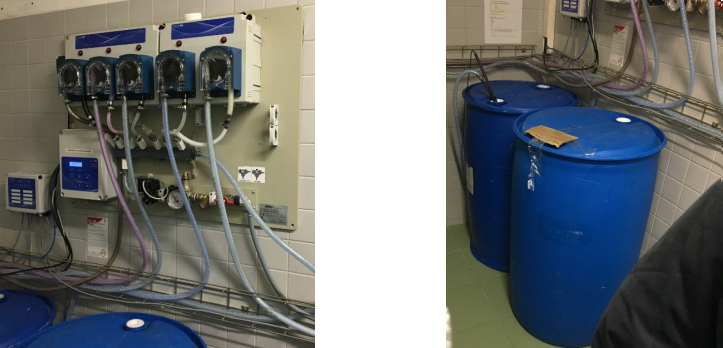
\includegraphics[scale=0.75]{etc/estrutura.png}
	\caption{Set of peristaltic pumps and storage reservoirs.}
	\label{fig:estruturaPNG}
\end{figure}

To keep all the washing machines operating without scarcity of laundry product is a real logistic problem. The misuse of laundry products during a washing cycle, e.g., liquid detergent, bleach, fabric softener, etc, present a major challenge to the \gls{SCMB} because of its direct impact on the quality of the service, waste water and electric energy and time reduction due the rerun of the washing machine cycle. 

As approached by Cemernek, Gursch and Kern \cite[p. 240]{CEMERNEK:2017}, it is unpredictable to say that all industrial laundry facilities have the same problem due the heterogeneity of the systems involved, but at the laundry's facility of the \gls{SCMB} concerns the logistic problem. The actual measurement system only detects when the reservoir is already empty, which may not be useful for the industrial laundry, as it may be necessary to rerun the washing cycle program in case the reservoirs are drain out in the middle of the process. Therefore, it can be solved trough the concepts of the new industrial era.


\section{Objectives}\label{cap:intro:objectives}



This work proposes a problem solution for industrial laundry system which consist in the development of an integrated system that is capable of monitoring and recording the detergent level inside of the reservoirs in the facilities of the Santa Casa da Misericórdia de Bragança (SCMB).

The project must be able to measure the liquid level using a low-cost ultrasonic sensor and the data must be collected using an ESP32 Development Board. The liquid-level information is sent to a MySQL DataBase using the Wi-Fi module which is integrated in the chip and it provides the client the real-time remote access of the information with the web based application development. Moreover, the microcontroller and the sensor must be integrated in a custom-made case which must adapt to the existing setup environment.

It is expected that the system provides a useful and reliable solution that monitors, logs and alerts the managements services in case of low detergent liquid-level, avoiding waste and ensuring the quality of the industrial laundry service.


\section{Document Structure}\label{cap:intro:document-sctruture}

This document is organized in 6 chapters, where the present chapter presents the contextualization, proposal and objectives of the work.

The Chapter \ref{cap:relatedWork} presents a bibliographic review, which address fundamental contents necessary to understand the concepts and understanding of the work.

Chapter \ref{cap:studyOfTools} provides an overview of ultrasonic sensors, demonstrating the method adopted for distance measurement, necessity of an embedded system and some basic characteristics about database and web development.

Chapter \ref{cap:development} starts with the presentation of the case study scenario, where the problem is explored and the solution adopted will be explained.

Chapter \ref{cap:results} presents the methodology used for testing and verifying the measurement system developed. Also, the influence of the temperature, battery performance and, overall considerations, regarding the solution adopted for the detergent supervision, are discussed. Moreover, the price list and the implementation of an \gls{IoT} Ecosystem for Industrial Washing Machines are presented.

Finally, the last chapter outlines the main conclusions and points out the future work.

